
\section{Bedienoberfläche}

Hier sollen die Skizzen/Prototypen von Bedienoberflächen dargestellt werden, als auch die Zusammenhänge zwischen denen (wie gelingt man von einem zu dem anderen Fenster/Ansicht). Ein Beispiel für Bildereinbau in LaTeX ist die Abbildung~\ref{gui:zusammenhang}.

\newcounter{gui}\setcounter{gui}{10}

\begin{description}[leftmargin=5em, style=sameline]	
	\begin{lhp}{gui}{GUI}{gui:zusammenhang}
		\item[Name:] Zusammenhänge
		\item[Beschreibung:] Zusammenhänge zwischen GUI-Ansichten
		\item[Relevante Systemfunktionen:] Alle
		\item[Abbildungen:] \ref{gui:zusammenhang}
	\end{lhp}
\end{description}

\begin{description}[leftmargin=5em, style=sameline]	
	\begin{lhp}{gui}{GUI}{gui:hauptseite}
		\item[Name:] Hauptseite
		\item[Beschreibung:] Hauptseite der Anwendung. Wird zur Navigation der Unterseiten verwendet
		\item[Relevante Systemfunktionen:] Nichts
		\item[Abbildungen:] \ref{gui:hauptseite}
	\end{lhp}
\end{description}

\begin{description}[leftmargin=5em, style=sameline]	
	\begin{lhp}{gui}{GUI}{gui:lobby}
		\item[Name:] Lobby
		\item[Beschreibung:] Lobby, in welcher sich die Spieler vor dem Spiel treffen und chatten können
		\item[Relevante Systemfunktionen:] \ref{funk:spielraum}\ref{funk:chat}\ref{funk:bots}
		\item[Abbildungen:] \ref{gui:lobby}
	\end{lhp}
\end{description}

\begin{description}[leftmargin=5em, style=sameline]	
	\begin{lhp}{gui}{GUI}{gui:spielfläche}
		\item[Name:] Spielfläche
		\item[Beschreibung:] Spielfläche auf welcher das Spiel ausgetragen wird.
		\item[Relevante Systemfunktionen:] \ref{funk:spielverw}\ref{funk:chat}\ref{funk:bots}
		\item[Abbildungen:] \ref{gui:spielfläche}
	\end{lhp}
\end{description}

\begin{description}[leftmargin=5em, style=sameline]	
	\begin{lhp}{gui}{GUI}{gui:bestenliste}
		\item[Name:] Bestenliste
		\item[Beschreibung:] Tabelle, auf welcher die Anzahl der Gewinne von Spielern angezeigt wird (geordnet nach Anzahl der Gewinne)
		\item[Relevante Systemfunktionen:] \ref{funk:bestenliste}
		\item[Abbildungen:] \ref{gui:bestenliste}
	\end{lhp}
\end{description}

\begin{description}[leftmargin=5em, style=sameline]	
	\begin{lhp}{gui}{GUI}{gui:einstellungen}
		\item[Name:] Einstellungen
		\item[Beschreibung:] Seite auf welcher Einstellungen verwaltet werden
		\item[Relevante Systemfunktionen:] \ref{funk:einstellung}
		\item[Abbildungen:] \ref{gui:einstellungen}
	\end{lhp}
\end{description}

\begin{description}[leftmargin=5em, style=sameline]	
	\begin{lhp}{gui}{GUI}{gui:login}
		\item[Name:] Login
		\item[Beschreibung:] Kleines Fenster, in welchem login daten angegeben werden, um sich in einen Account einzuloggen
		\item[Relevante Systemfunktionen:] \ref{funk:zugriff}
		\item[Abbildungen:] \ref{gui:login}
	\end{lhp}
\end{description}

\begin{figure}
	\centering
	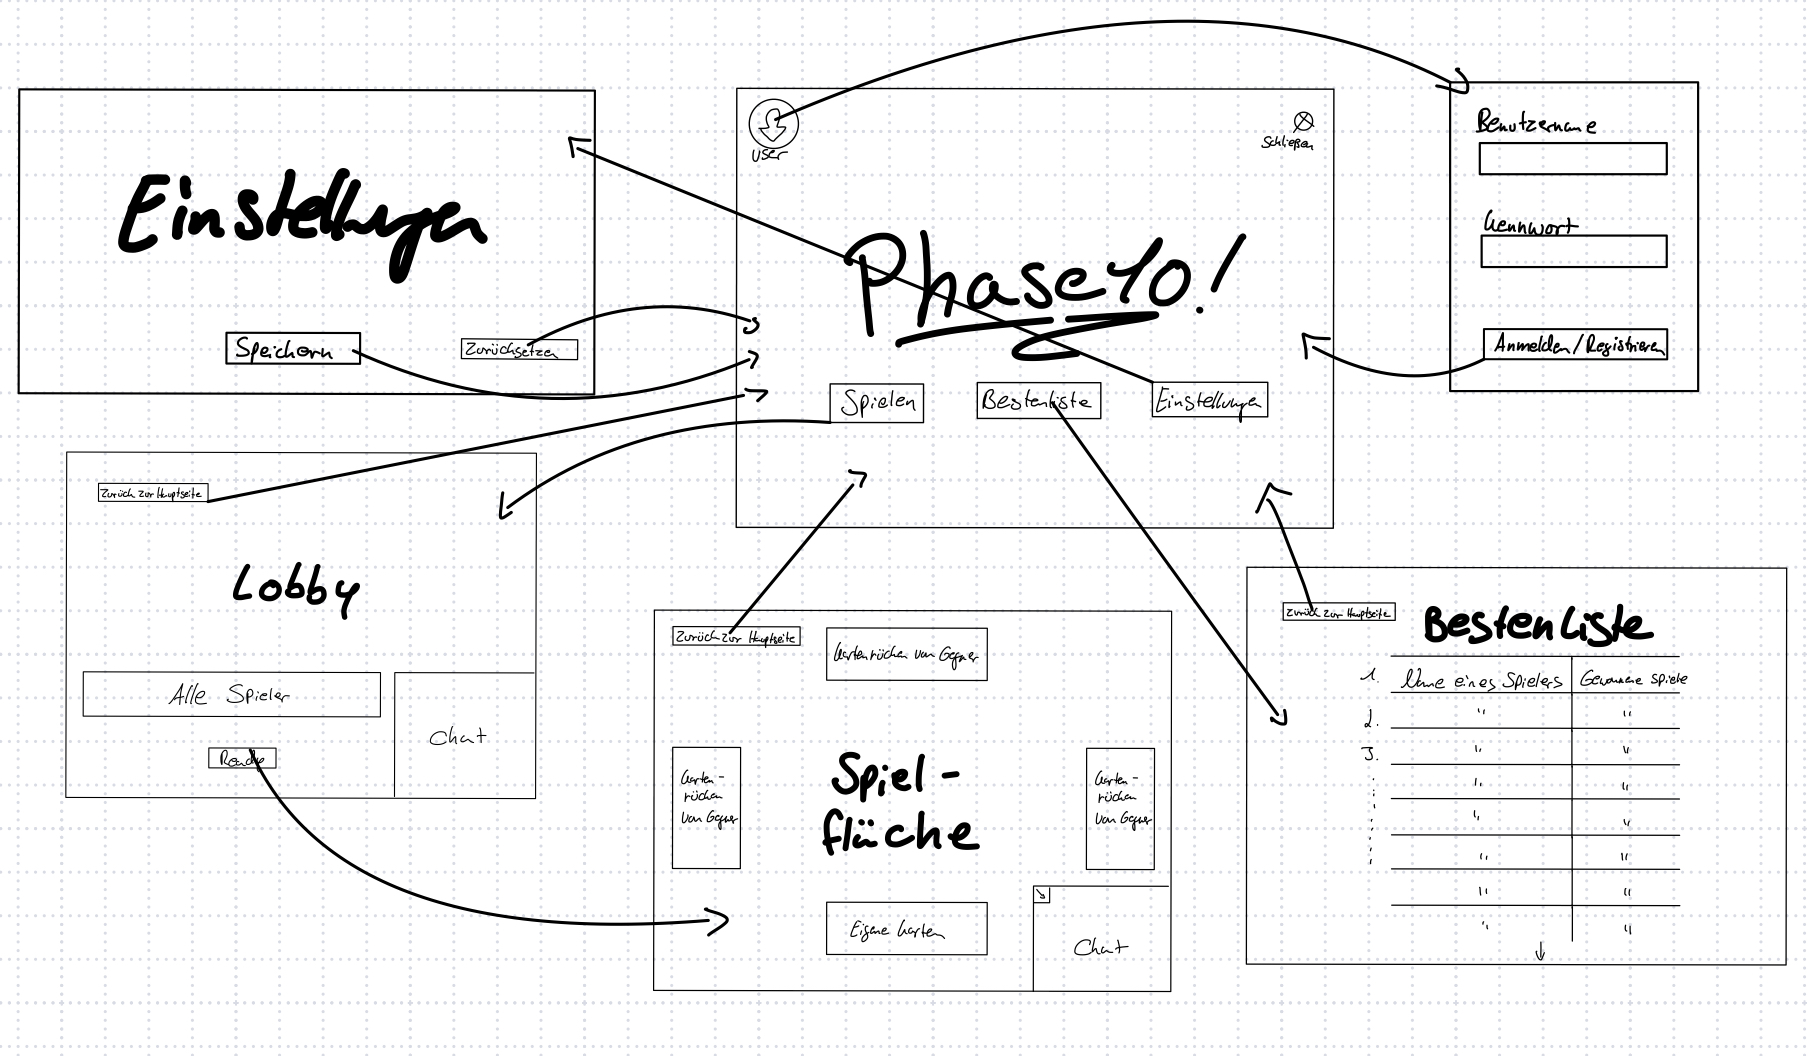
\includegraphics[width=0.9\textwidth]{img/gui-zusammenhang}
	\caption{Darstellung der Zusammenhänge zwischen GUI-Ansichten.}
	\label{gui:zusammenhang}
\end{figure}

\begin{figure}
	\centering
	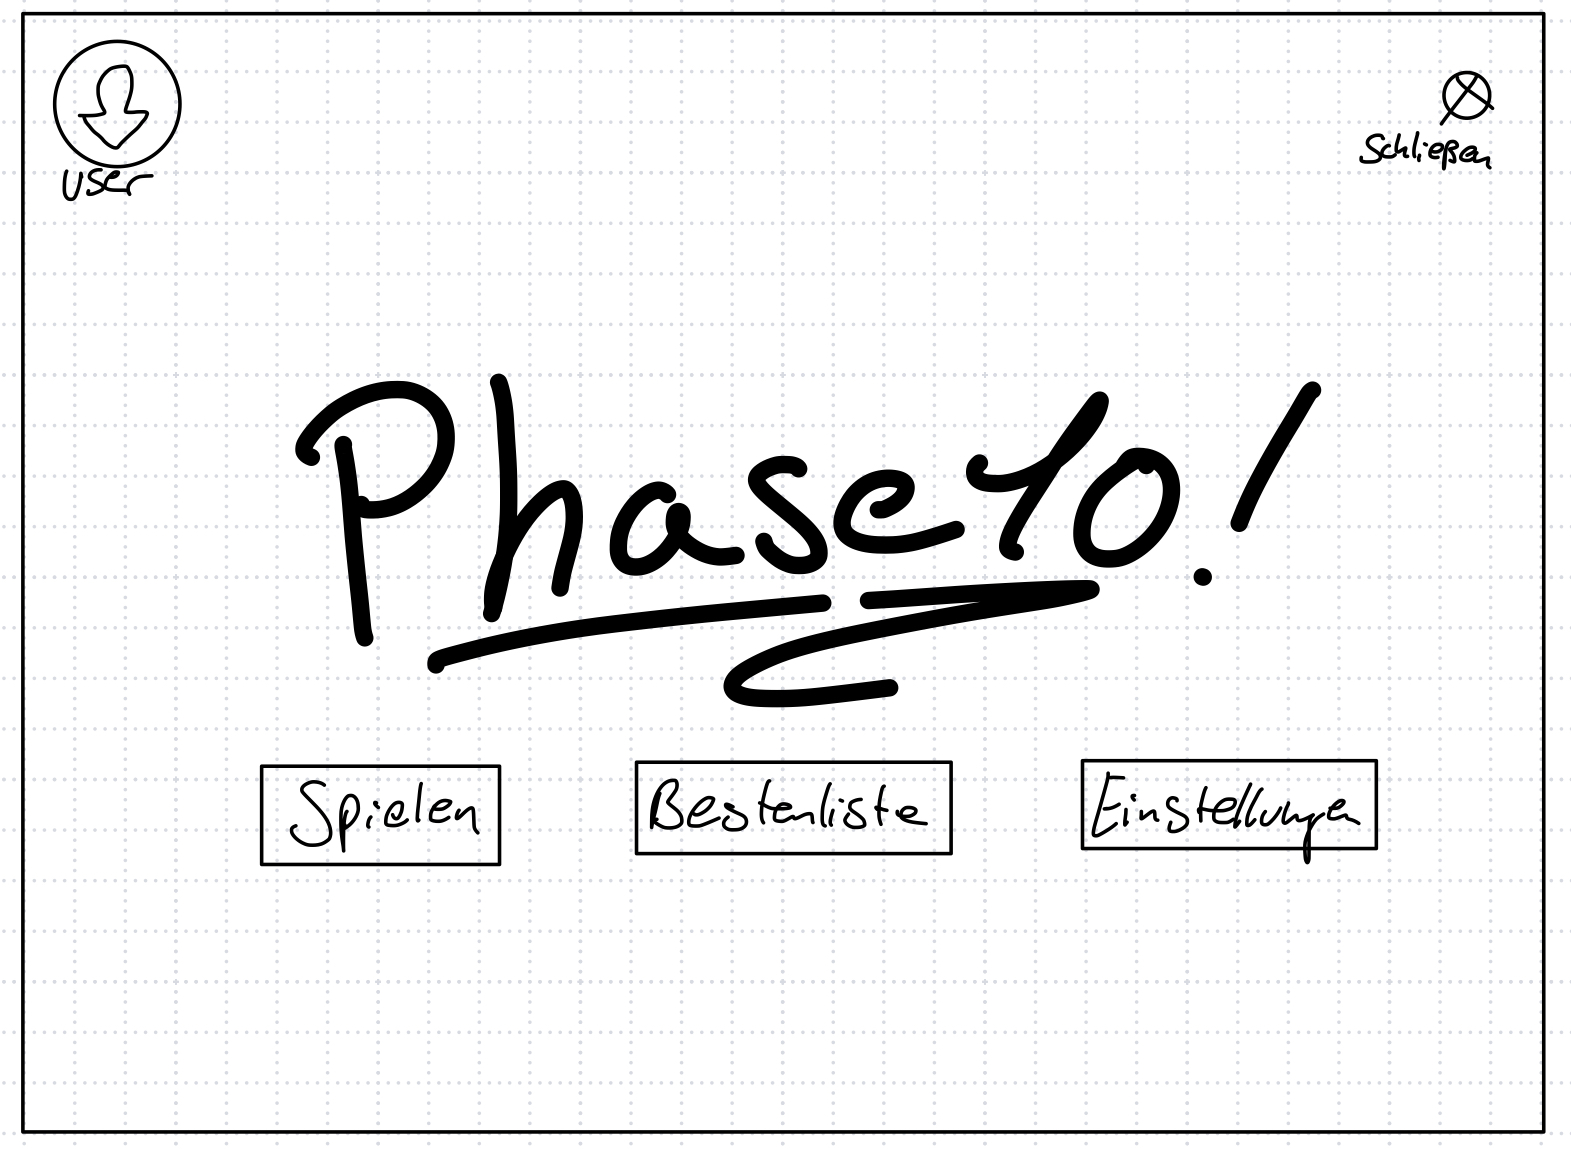
\includegraphics[width=0.9\textwidth]{img/hauptseite.jpeg}
	\caption{Beispiel für ein GUI-Mockup. Dieser Text ist auch nur ein Beispiel :)}
	\label{gui:hauptseite}
\end{figure}

\begin{figure}
	\centering
	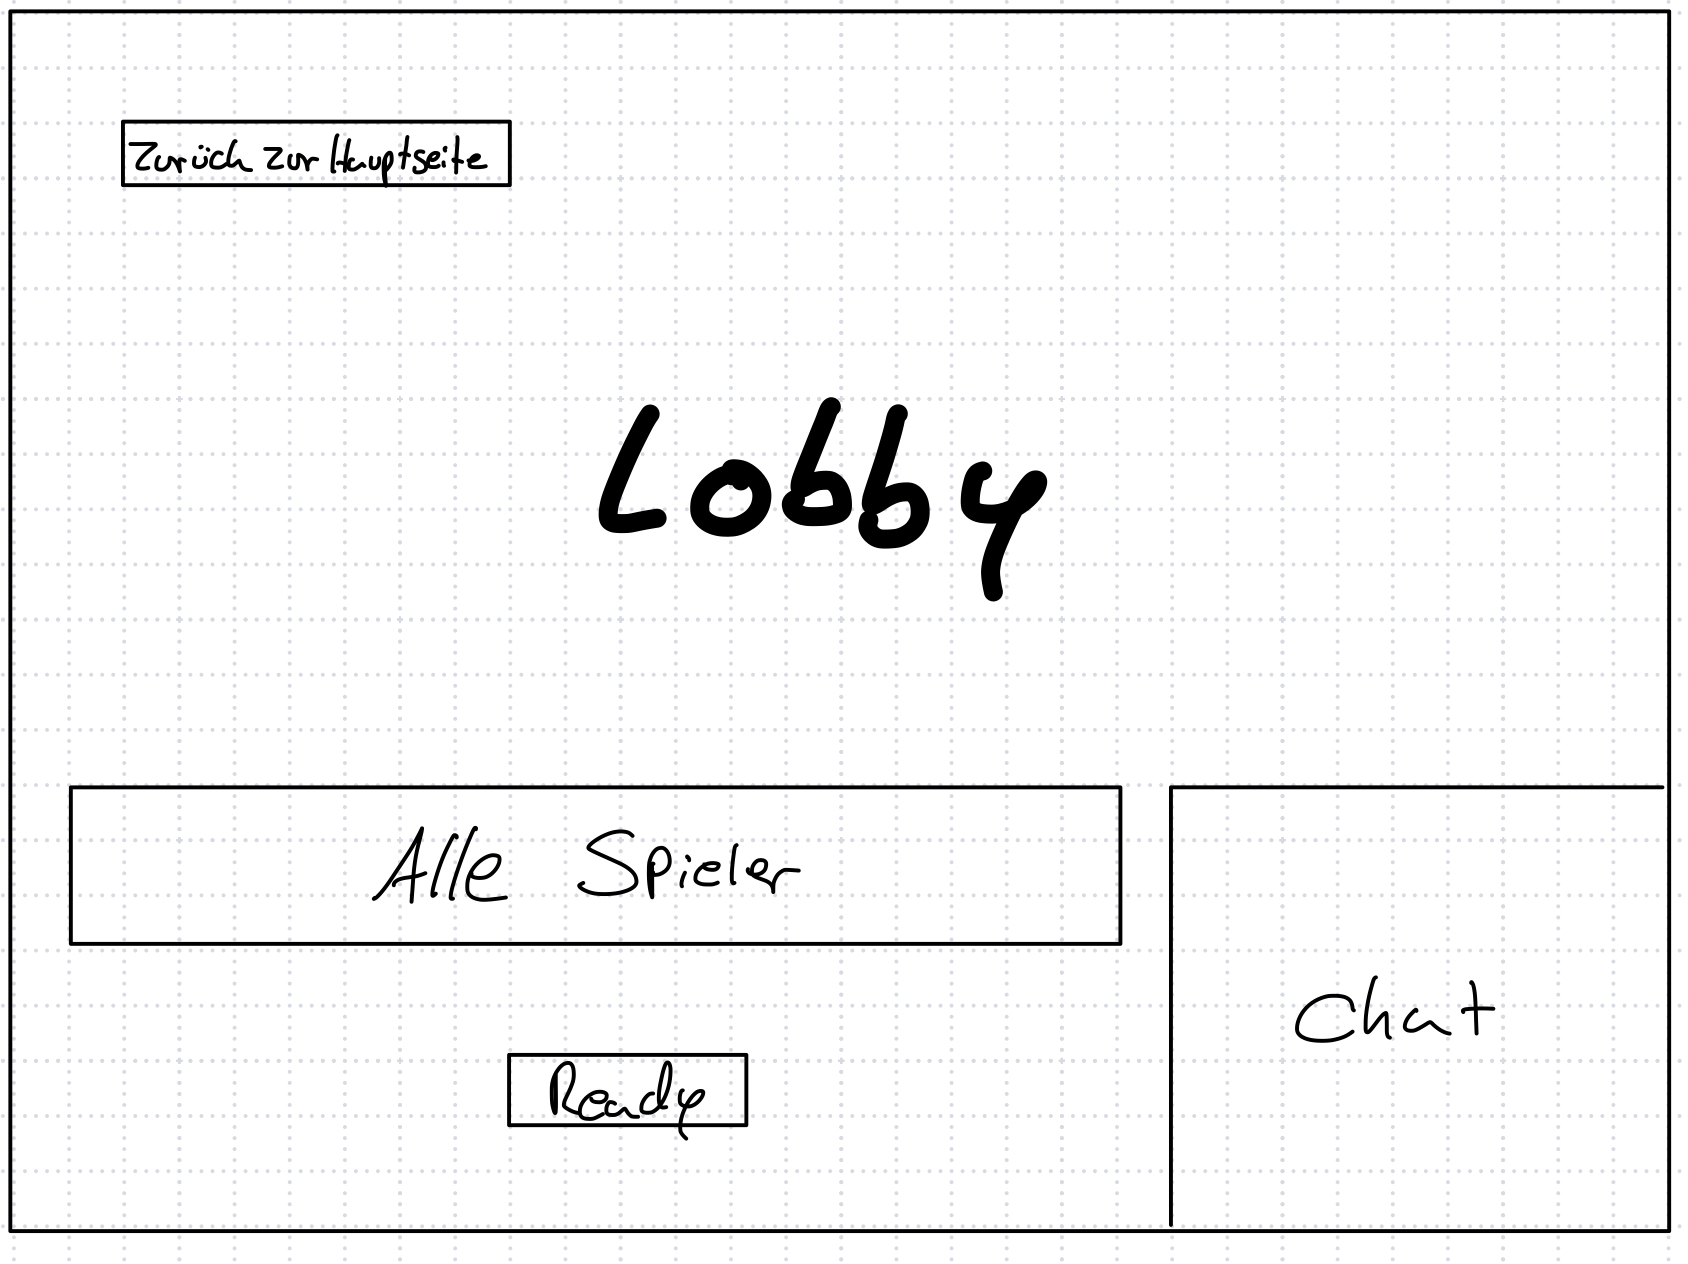
\includegraphics[width=0.9\textwidth]{img/lobby}
	\caption{Beispiel für ein GUI-Mockup. Dieser Text ist auch nur ein Beispiel :)}
	\label{gui:lobby}
\end{figure}

\begin{figure}
	\centering
	\includegraphics[width=0.9\textwidth]{img/spielfläche}
	\caption{Beispiel für ein GUI-Mockup. Dieser Text ist auch nur ein Beispiel :)}
	\label{gui:spielfläche}
\end{figure}

\begin{figure}
	\centering
	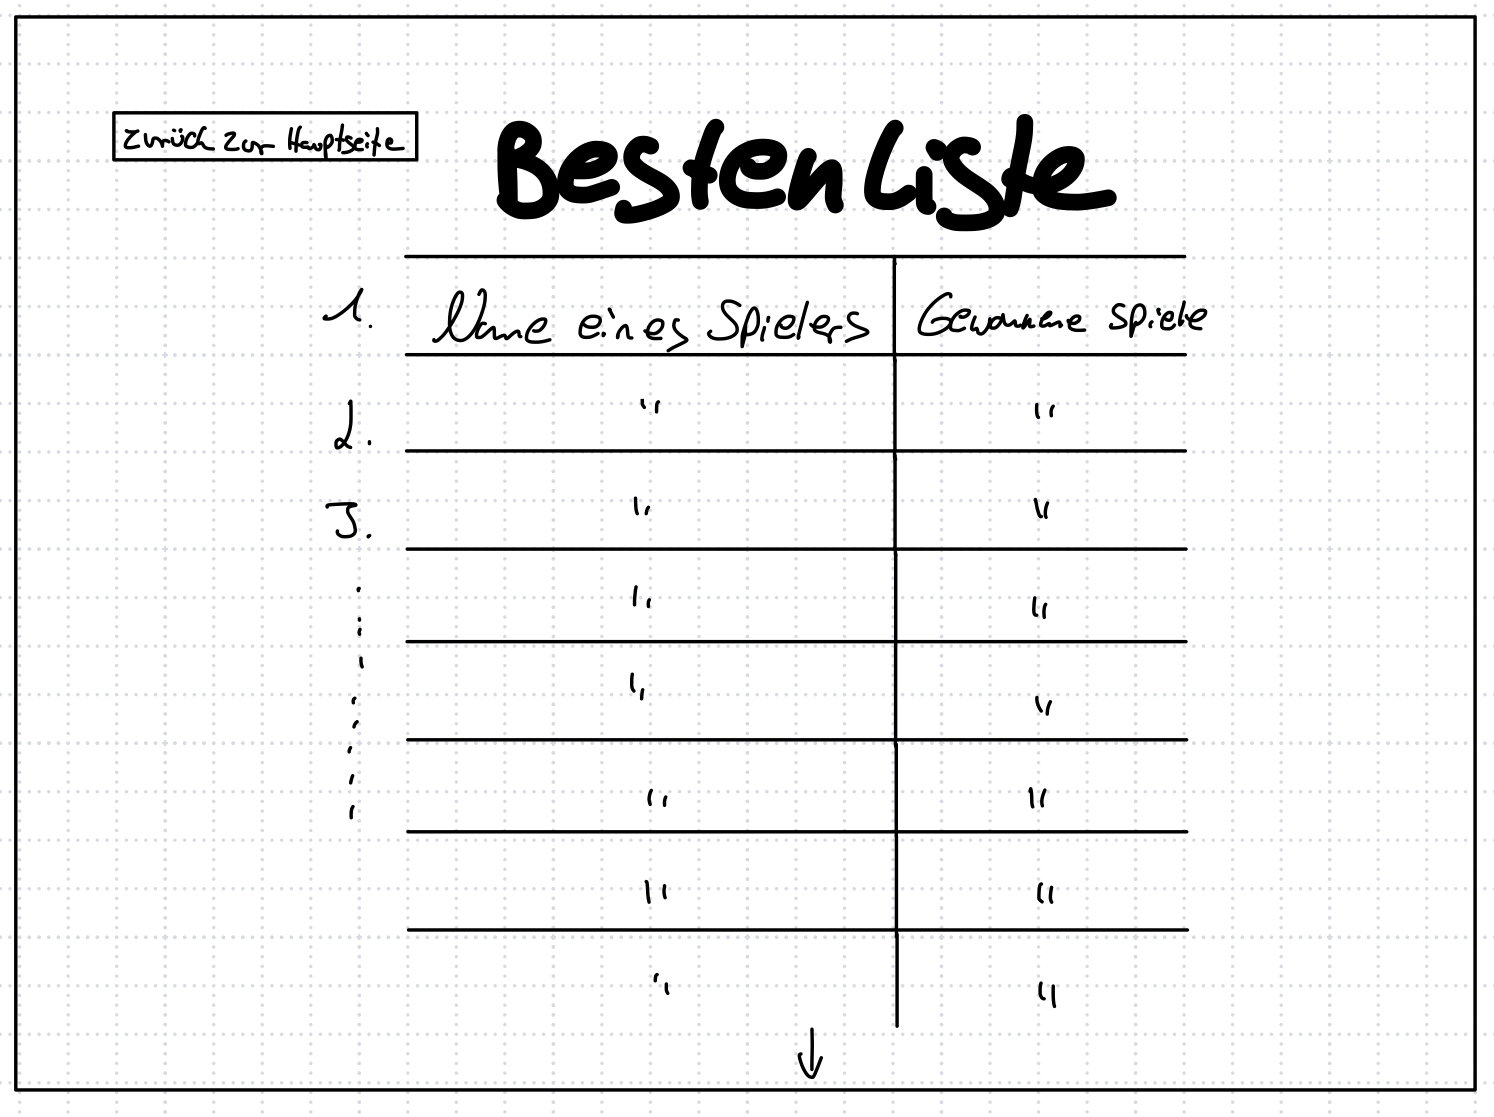
\includegraphics[width=0.9\textwidth]{img/bestenliste}
	\caption{Beispiel für ein GUI-Mockup. Dieser Text ist auch nur ein Beispiel :)}
	\label{gui:bestenliste}
\end{figure}

\begin{figure}
	\centering
	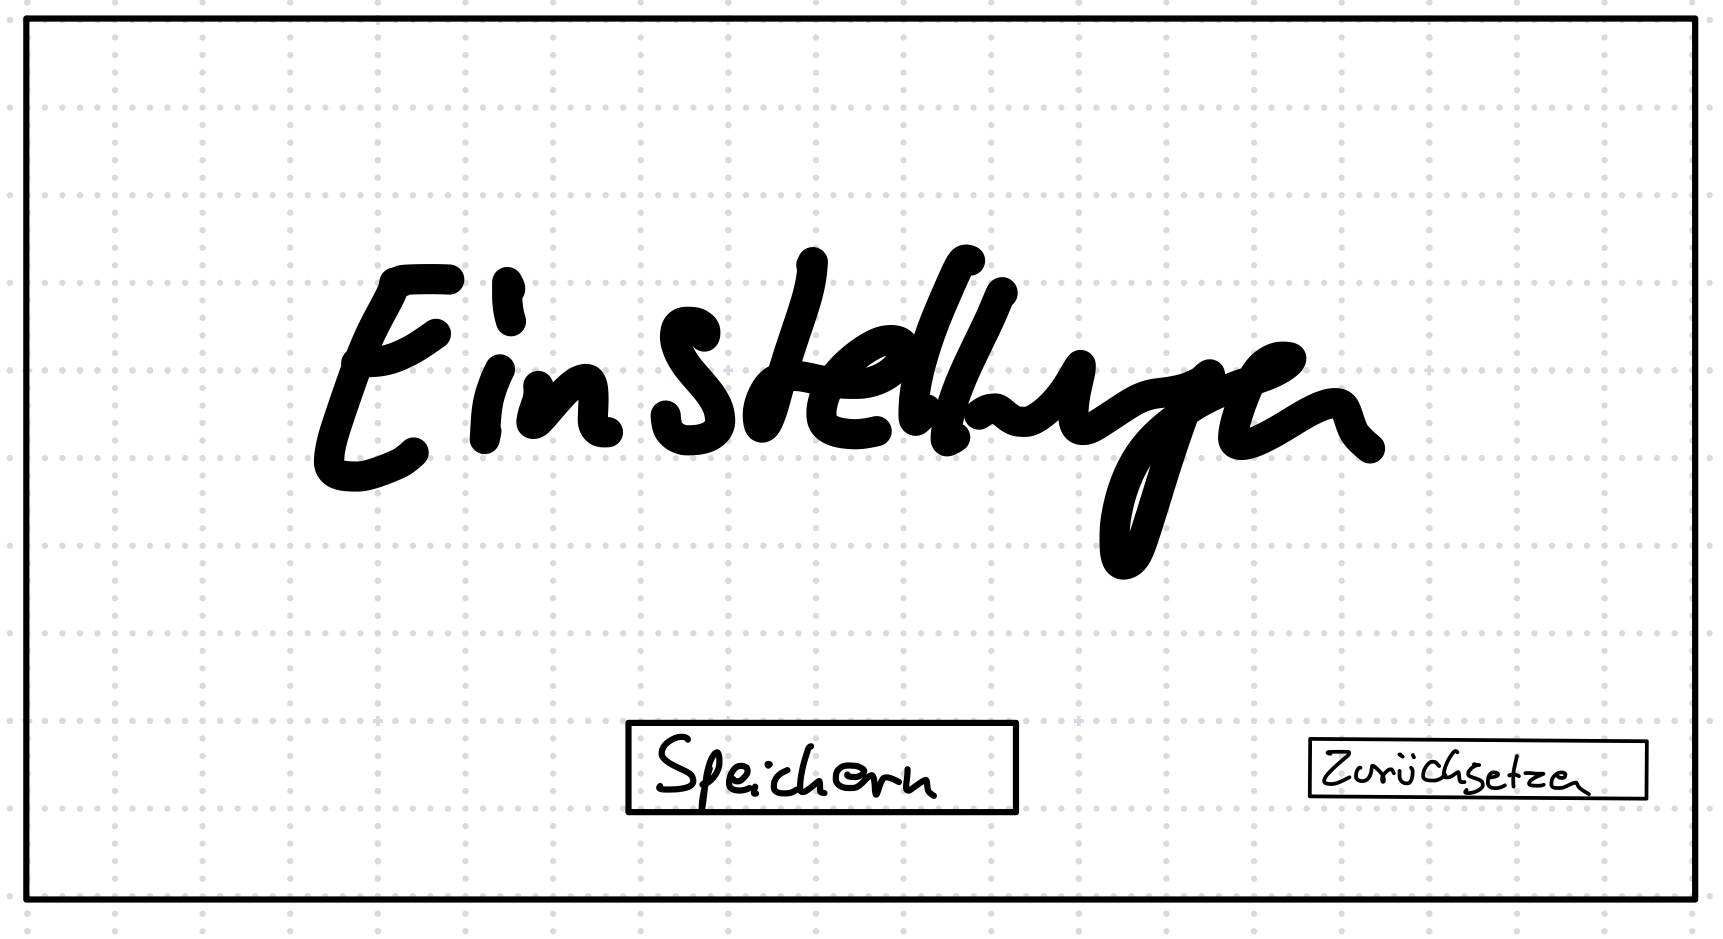
\includegraphics[width=0.9\textwidth]{img/einstellungen}
	\caption{Beispiel für ein GUI-Mockup. Dieser Text ist auch nur ein Beispiel :)}
	\label{gui:einstellungen}
\end{figure}

\begin{figure}
	\centering
	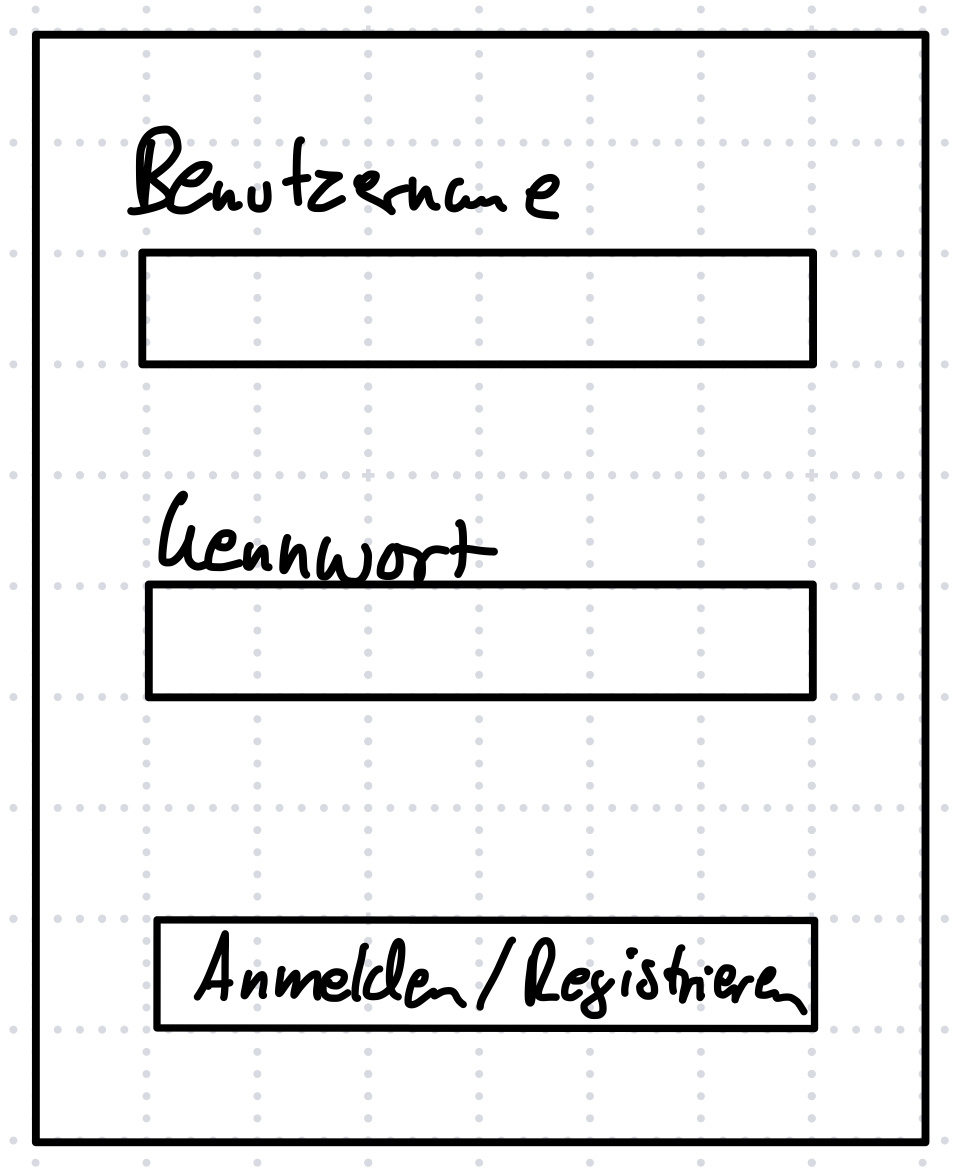
\includegraphics[width=0.9\textwidth]{img/login}
	\caption{Beispiel für ein GUI-Mockup. Dieser Text ist auch nur in Beispiel :)}
	\label{gui:login}
\end{figure}